\section{Controles}

La excavadora tiene los siguientes controladores asociados a un hueso:

\begin{itemize}
    \item \textbf{Rotación de toda la plataforma: }Permite rotar la excavadora sobre el eje Z, de manera que pueda girar sin tener que moverse del sitio.
    
    % foto del controlador y algunas del movimiento
    \begin{figure}[H]
        \centering
        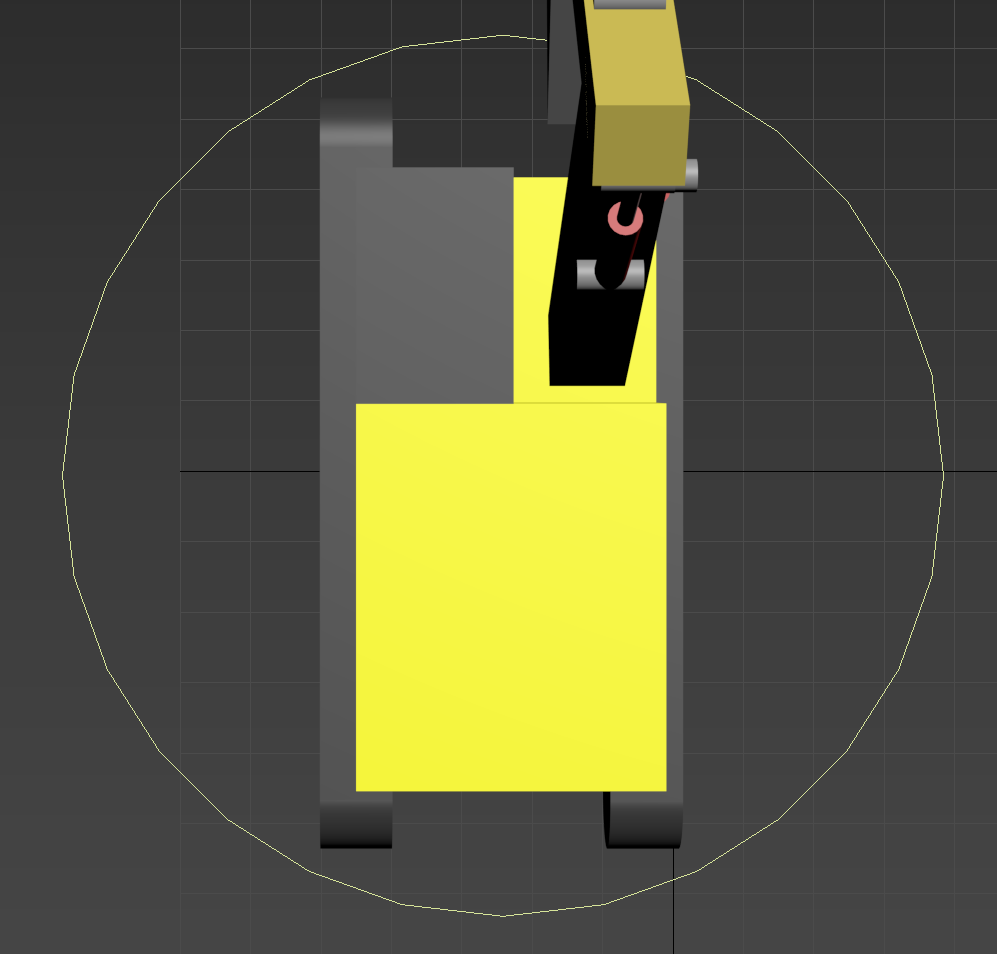
\includegraphics[width=0.5\textwidth]{imagenes/controlplat.png}
        \caption{Controlador de la plataforma.}
     \end{figure}

     \newpage

    \item \textbf{Rotación del brazo: }Permite rotar la primera pieza del brazo que sale de la base de la excavadora.
    
    % foto del controlador y dos del movimiento
    \begin{figure}[H]
        \centering
        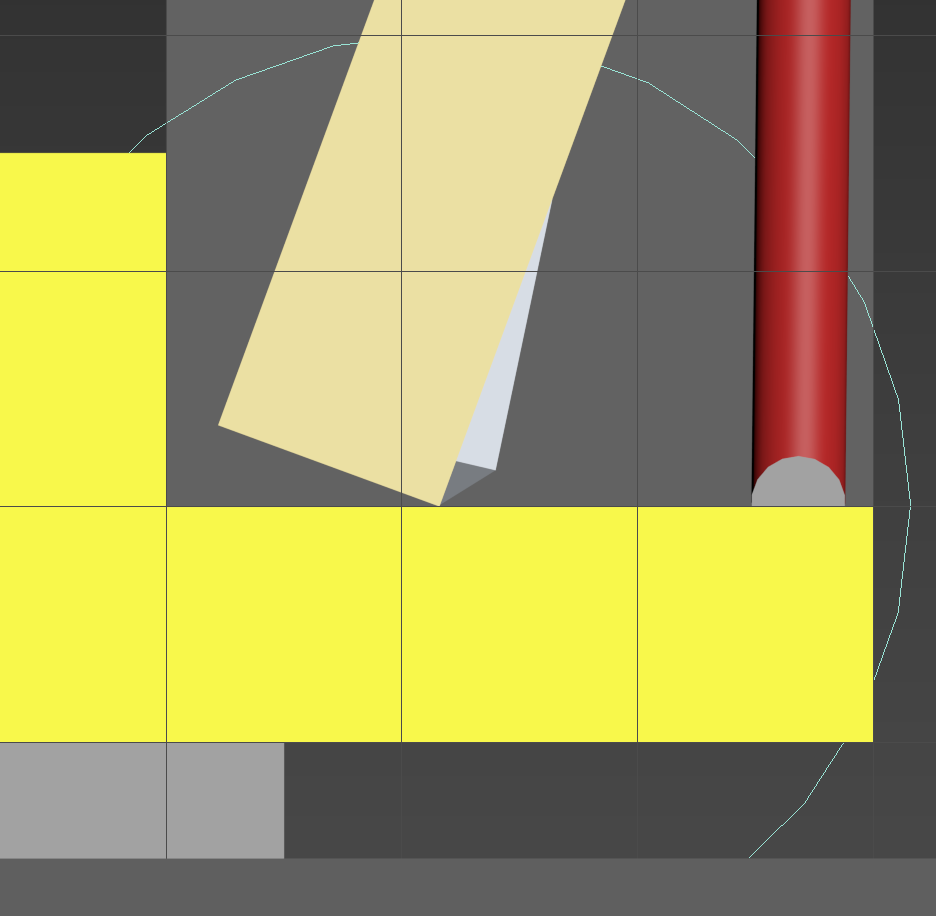
\includegraphics[width=0.5\textwidth]{imagenes/brazo1control.png}
        \caption{Controlador del brazo.}
     \end{figure}    

    \item \textbf{Rotación del segundo brazo: }Permite rotar la segunda pieza del brazo, conectada a la pieza anterior.
    
    % lo mismo que antes
    \begin{figure}[H]
        \centering
        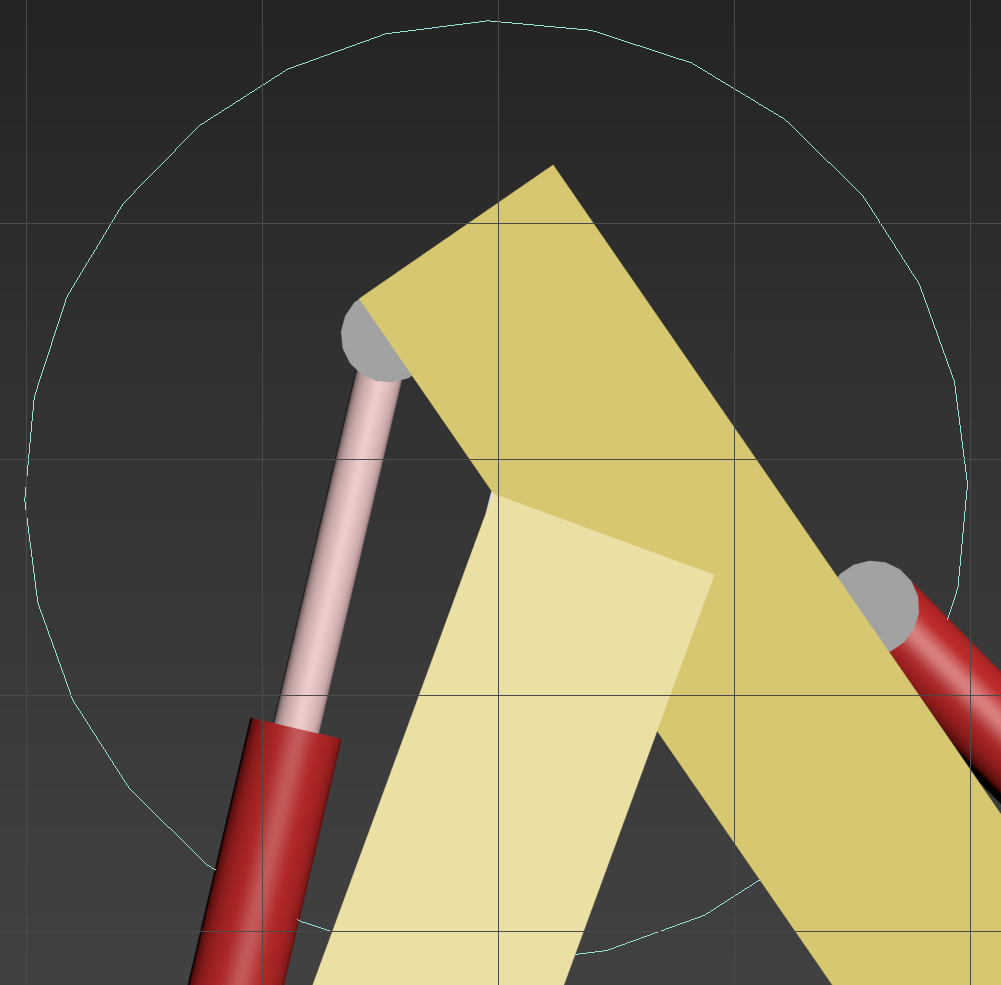
\includegraphics[width=0.5\textwidth]{imagenes/brazo2control.png}
        \caption{Controlador del segundo brazo.}
     \end{figure}    

     \newpage

    \item \textbf{Rotación de la pala: }Permite rotar la pala de la excavadora.
    \begin{figure}[H]
        \centering
        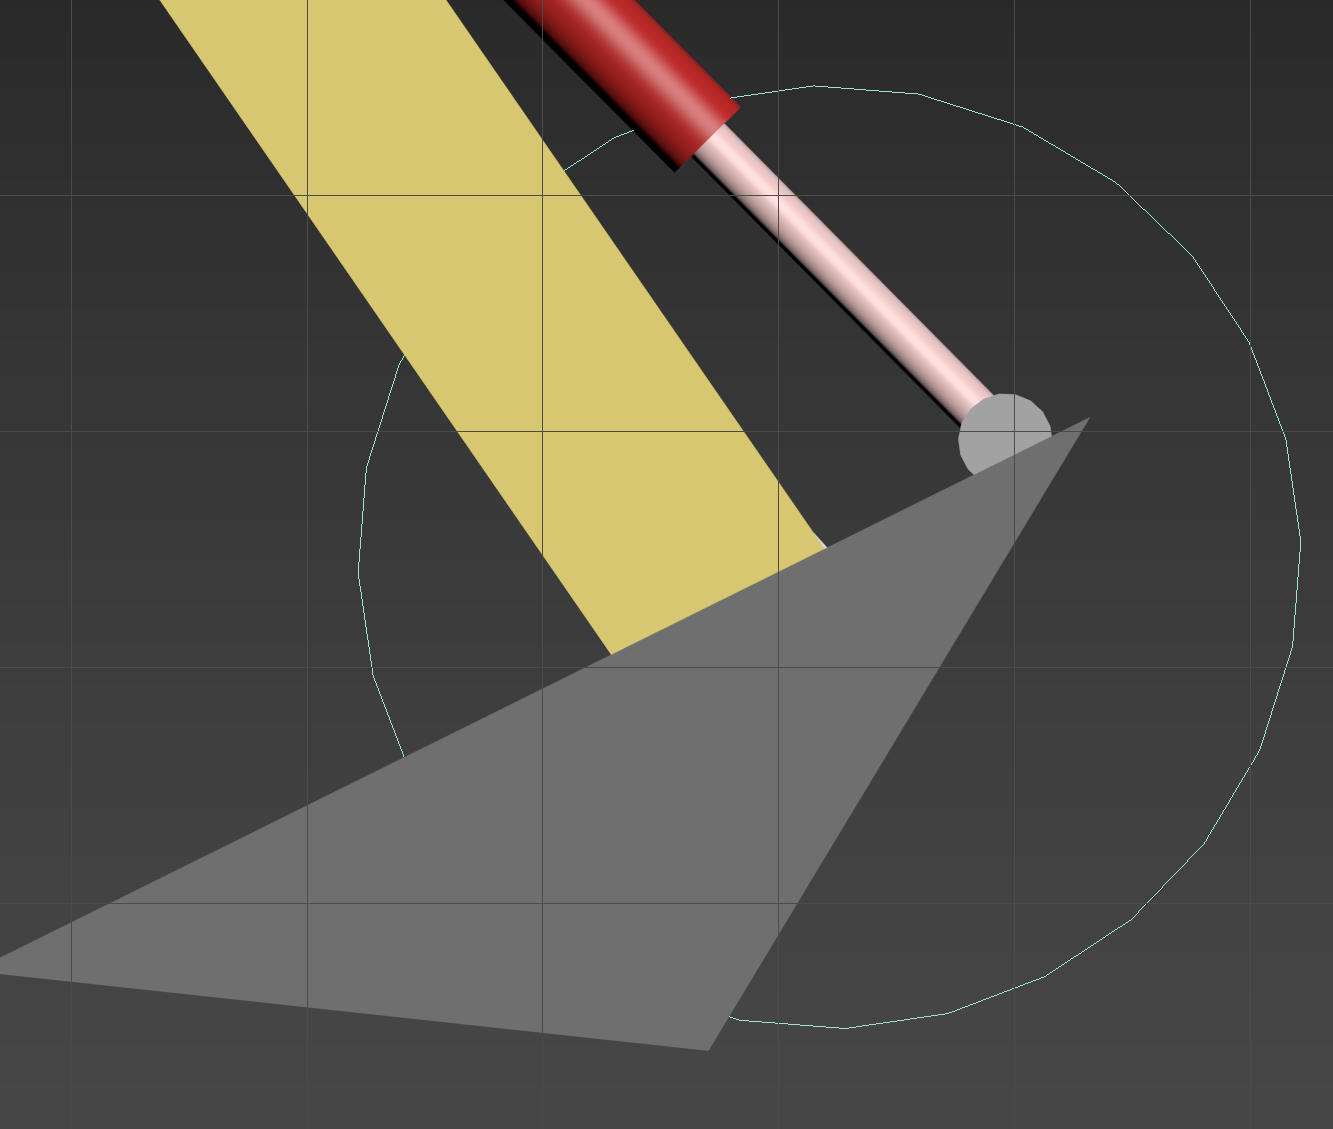
\includegraphics[width=0.5\textwidth]{imagenes/palacontrol.png}
        \caption{Controlador de la pala.}
     \end{figure}        
\end{itemize}

\bigskip

Además, para tener un control más cómodo y preciso, he añadido la siguiente interfaz:

% interfaz de eso
\begin{figure}[H]
    \centering
    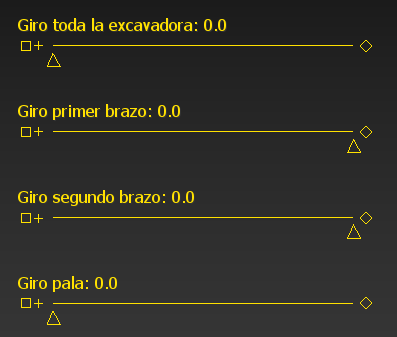
\includegraphics[width=0.5\textwidth]{imagenes/sliders.png}
    \caption{Interfaz para el control de la excavadora.}
 \end{figure}
 

Esta interfaz está compuesta de \textit{sliders} que controlan los controladores (valga la redundancia) mediante \textit{Wire parameters} del valor actual del \textit{slider}, con el eje de rotación correspondiente.

\bigskip

Cabe destacar que los valores de rotación en los que trabajan los \textit{sliders} son en radianes. Se podría haber arreglado y haberle aplicado una función para que apareciese en grados sexagesimales, pero me he dado cuenta cuando tenía la animación terminada, haciendo que tuviera que realizarla de nuevo.

\newpage